\documentclass{article}
\usepackage{amsmath,amsthm,amsfonts,amssymb,amscd}
\usepackage{fullpage}
\usepackage{lastpage}
\usepackage{enumerate}
\usepackage{fancyhdr}
\usepackage[percent]{overpic}
\usepackage{mathrsfs}
\usepackage{wrapfig}
\usepackage{multirow}
\usepackage{placeins}
\usepackage{amsmath}
\usepackage{amssymb}
\usepackage{amscd}
\usepackage{lscape}
\usepackage{graphicx}
\usepackage[usenames,dvipsnames]{color}
\usepackage{listings}
\usepackage[usenames,dvipsnames,svgnames,table]{xcolor}
\usepackage[left=2cm,right=2cm,top=2.5cm,bottom=2.5cm, headsep = 0.9cm]{geometry}
\usepackage{verbdef}
\usepackage[UKenglish]{isodate}
\usepackage{enumitem}
\setenumerate{listparindent=\parindent}
\cleanlookdateon%
\setlength{\parindent}{0.0in}
\setlength{\parskip}{0.0in}
\usepackage{setspace}
\definecolor{gray}{RGB}{90,90,90}
\usepackage[colorlinks=true, linktoc=all, linkcolor=blue]{hyperref}
\usepackage{fancyvrb}
\newcommand{\paren}[1]{\left(#1\right)}
\newcommand{\sqbracket}[1]{\left[#1\right]}
\newcommand{\cbracket}[1]{\left\{#1\right\}}
\newcommand\numberthis{\addtocounter{equation}{1}\tag{\theequation}}
\newcommand{\var}{\text{var}}
\newcommand{\cov}{\text{cov}}
\newcommand{\expit}{\text{expit}}
\newcommand{\abs}[1]{\left\lvert#1\right\rvert}
\setlength\parindent{10pt}

\pagestyle{fancy}
\fancyhf{}
\setlength{\headheight}{12pt}
\fancyhead[L]{BIOST 561, Autumn 2016}
\fancyhead[R]{Homework 6 - KEY}
\fancyhead[C]{17 November 2016}
\fancyfoot[C]{\thepage}
\begin{document}
Suppose that, as in lecture, we have a sample of $n$ observations generated from the model
\begin{align*}
X_i &\stackrel{i.i.d.}{\sim} N(0, 1), \\
u_i &\stackrel{i.i.d.}{\sim} N(0, 1), \text{ independent of the } X_i, \\
Y_i \mid X_i, u_i &= \beta_0 + \beta_1 X_i + \epsilon_i, \text{ where} \\
\epsilon_i &= \abs{X_i}u_i.
\end{align*}
In this assignment we will compare model-based, robust (``sandwich''), and bootstrap standard errors for estimates $\hat{\beta}_1$ of $\beta_1$ from linear regression models. We set $\beta_0 = 1$ and $\beta_1 = 2$.
\begin{enumerate}
\item For $n \in \{10, 100, 1000\}$, conduct a simulation that compares the three different standard error estimates (model-based, sandwich, bootstrap) of the true standard error of $\hat{\beta}$. In each simulation, you will need to replicate the following steps $B = 5000$ times:
\begin{enumerate}
\item Generate a sample of observations $(X_i, Y_i)$ of size $n$ according to the model above
\item Fit a linear regression model to the observed data and record the estimate $\hat{\beta}_1$
\item Compute model-based and robust standard errors for $\hat{\beta}_1$
\item Compute a bootstrap standard error for $\hat{\beta}_1:$ 
\begin{itemize}
\item Draw 1000 bootstrap samples of size $n$ from the observed sample $(X, Y)$
\item Compute $\hat{\beta}_1$ for each of these 1000 samples
\item Compute the standard deviation of these bootstrapped coefficient estimates
\end{itemize}
\end{enumerate}
You can use the function \texttt{doOne()} in the file \texttt{se\_ex1.R} as a starting point for your simulations. You may do this on your own machine or on \texttt{cox}. Write your code so that the results are reproducible.

\item[Answer:] See Appendix, \texttt{se\_ex1.R} and \texttt{submit\_ex1\_cox.sh}. This job took many hours to run, since \texttt{cox} had to run all 5000 replications of each job before finishing.

\item Conduct simulations using 3 additional values of $n$, of your choosing, this time using batch submission of jobs on \texttt{bayes}. Split each simulation into either 5 or 10 jobs (not 1 job and not 5000 individual jobs). Perform this batch submission either using a loop in your shell script, or by using a job array. \textbf{NB}: If \texttt{bayes} is full, \texttt{gosset} has an identical setup (i.e. use \texttt{qsub} to submit jobs) and is restricted to student use only. This is an older (i.e. slower) cluster, but often has available cores.

\item[Answer:] See Appendix, \texttt{se\_ex2.R}, \texttt{call\_ex2\_once.sh}, and \texttt{submit\_ex2\_batch.sh}. These jobs took 1.5 hours total to run, since \texttt{gosset} was able to run many jobs simultaneously. Note that \texttt{bayes} would have likely gotten the job done more quickly.

\item Present your results graphically and/or tabularly in a way that best illustrates your findings. Comment on what you see. Attach your code and any scripts in an Appendix.

\item[Answer:] Table \ref{output_mat} contains the results of our simulation study. We chose additional values of $n$ to be 50, 300, and 500, yielding a total of 6 sample sizes. All results are based on 5000 replications. Note that we also present the results graphically in Figure \ref{output_plot} --- this is only one way to present these results, and is not required if you chose to present the results in a table. 

We see that for all sample sizes, the estimate of $\hat{\beta}$ is close to the truth. We could expect this to happen, since the heteroskedasticity does not affect our point estimate but rather our standard error estimates. This is shown in the table as well --- the model-based standard errors do not achieve the nominal 95\% coverage for any value of sample size. However, if we use robust standard error estimates or the bootstrap, we get much closer to the nominal 95\% coverage even for small $n$. As we would expect, more observations yields better coverage for confidence intervals based on the bootstrap or sandwich standard error estimates. 

The most interesting finding is that the bootstrap appears to outperform sandwich standard error estimates for small $n$. This seems reasonable, given that the bootstrap is approximating the sampling distribution of $\hat{\beta}$ and using this to yield a standard error estimate, while the sandwich estimator uses only the original data. The fact that the performance of the two is comparable for large sample size means that the sandwich standard error estimator relies more heavily on a large sample size than does the bootstrap. However, it does take significantly longer to compute bootstrap standard error estimates than sandwich standard error estimates.

\begin{table}[ht]
\centering
\caption{Estimated coefficients and nominal coverage of 95\% confidence intervals for different sample sizes, based on 5000 replications.}
\begin{tabular}{rrrrrr}
  \hline
  & & \multicolumn{3}{c}{Standard error estimation method} \\
 & $\hat{\beta}$ & Model & Sandwich & Bootstrap & $n$ \\ 
  \hline
1 & 2.004 & 0.716 & 0.727 & 0.850 & 10.000 \\ 
  2 & 1.996 & 0.751 & 0.906 & 0.911 & 50.000 \\ 
  3 & 2.001 & 0.733 & 0.919 & 0.920 & 100.000 \\ 
  4 & 2.000 & 0.740 & 0.943 & 0.943 & 300.000 \\ 
  5 & 2.002 & 0.740 & 0.944 & 0.945 & 500.000 \\ 
  6 & 2.000 & 0.744 & 0.953 & 0.952 & 1000.000 \\ 
   \hline
\end{tabular}
\label{output_mat}
\end{table}

\begin{figure}[ht]
\centering
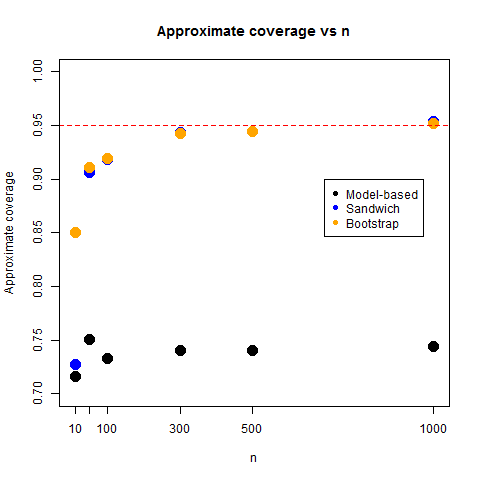
\includegraphics[width = .5\textwidth]{cover_by_n.png}
\caption{Approximate coverage of nominal 95\% confidence intervals --- based on 5000 replications --- versus sample size, for the three types of standard error estimates.}
\label{output_plot}
\end{figure}

\FloatBarrier
\item[Appendix:] Here is the code that I used for the assignment. Note that many of these functions could be different, and definitely will be if you chose to do (2) using a loop in your shell script. I have also attached my code to load all of the data and create plots at the end.

{\fontsize{9pt}{7.2}\selectfont
\begin{verbatim}
[brianw26@cox ~/biost_561]$ more submit_ex1_cox.sh
#!/bin/sh

Rscript se_ex1.R n=10 truebeta=2 seed=147 B=5000 &
Rscript se_ex1.R n=100 truebeta=2 seed=247 B=5000 &
Rscript se_ex1.R n=1000 truebeta=2 seed=347 B=5000

#!/usr/local/bin/Rscript


#########################################################################
##
## FILE: se_ex1.R
##
## CREATED: 27 October 2016 by Brian Williamson
##
## PURPOSE: Robust SE example for BIOST 561
##
## UPDATES:
## DDMMYY INIT COMMENTS
## ------ ---- --------
## 171116 BDW  Added bootstrap functionality
#########################################################################
args <- commandArgs(TRUE)
## Parse the arguments
if(length(args) == 0) {
  print("No arguments supplied.")
} else {
  for (i in 1:length(args)) {
    eval(parse(text = args[i]))
  }
}
if(!exists("truebeta")) {
  truebeta <- 2
  cat("\n Note: Assmuming truebeta = 2 \n")
}
if(!exists("n")) {
  n <- 500
  cat("\n Note: Setting n = 500 \n")
}
if(!exists("seed")) {
  seed <- 547
  cat("\n Note: Setting seed = 547 \n")
}
if(!exists("B")) {
  B <- 1000
  cat("\n Note: setting B = 1000 \n")
}

## Function to perform a bootstrap
## Args: data - the dataset to bootstrap on
##          b - the number of bootstrap samples
## Returns: the b bootstrap datasets, as a list
myBootstrap <- function(data, b){
  boot <- list()
  if (is.vector(data)) {
    for (i in 1:b) {
      samp <- sample(seq_len(length(data)), length(data), replace = TRUE)
      bootb <- data[samp]
      boot[[i]] <- bootb
    }
  } else {
    for (i in 1:b) {
      samp <- sample(seq_len(nrow(data)), nrow(data), replace = TRUE)
      bootb <- data[samp,]
      boot[[i]] <- bootb
    }
  }
  return(boot)
}

## Function to run the simulation once
doOne <- function(n, beta) {
  ## create the data
  x <- rnorm(n, 0, 1)
  u <- rnorm(n, 0, 1)
  eps <- abs(x)*u
  beta0 <- 1
  y <- beta0 + beta*x + eps
  
  ## create the bootstrap datasets
  boot <- myBootstrap(data.frame(x, y), b = 1000)
  ## get the estimates
  betahats <- unlist(lapply(boot, function(x) coefficients(lm(y ~ ., data = x))[2]))
  
  ## fit the linear regression model
  mod <- lm(y ~ x)
  
  ## extract model coefficients and SEs
  est <- coefficients(mod)[2]
  se <- vector("numeric", 3)
  se[1] <- sqrt(diag(vcov(mod)))[2]
  se[2] <- sqrt(diag(vcovHC(mod, "HC0")))[2]
  se[3] <- sd(betahats)
  
  ## Create CIs
  ci <- est + se %o% qnorm(c(0.025, 0.975))
  cover <- beta > ci[, 1] & beta < ci[, 2]
  names(cover) <- c("Model", "Sandwich", "Bootstrap")
  
  ## return
  return(c(est, cover))
}

library(sandwich)
set.seed(seed)
system.time(output <- replicate(B, doOne(n = n, beta = truebeta)))
apply(output, 1, mean)


[brianw26@bayes0 ~/biost_561]$ more submit_ex2_batch.sh
#!/bin/sh

qsub -t 1-15 -cwd -e iotrash/ -o iotrash/ -shell no -b yes -m e ./call_ex2_once.
sh

[brianw26@bayes0 ~/biost_561]$ more call_ex2_once.sh
#!/bin/sh

Rscript se_ex2.R

#!/usr/local/bin/Rscript


#########################################################################
##
## FILE: se_ex2.R
##
## CREATED: 27 October 2016 by Brian Williamson
##
## PURPOSE: Robust SE example for BIOST 561
##
## UPDATES:
## DDMMYY INIT COMMENTS
## ------ ---- --------
## 171116 BDW  Added bootstrap functionality
#########################################################################

## Function to perform a bootstrap
## Args: data - the dataset to bootstrap on
##          b - the number of bootstrap samples
## Returns: the b bootstrap datasets, as a list
myBootstrap <- function(data, b){
  boot <- list()
  if (is.vector(data)) {
    for (i in 1:b) {
      samp <- sample(seq_len(length(data)), length(data), replace = TRUE)
      bootb <- data[samp]
      boot[[i]] <- bootb
    }
  } else {
    for (i in 1:b) {
      samp <- sample(seq_len(nrow(data)), nrow(data), replace = TRUE)
      bootb <- data[samp,]
      boot[[i]] <- bootb
    }
  }
  return(boot)
}

## Function to run the simulation once
doOne <- function(n, beta) {
  ## create the data
  x <- rnorm(n, 0, 1)
  u <- rnorm(n, 0, 1)
  eps <- abs(x)*u
  beta0 <- 1
  y <- beta0 + beta*x + eps
  
  ## create the bootstrap datasets
  boot <- myBootstrap(data.frame(x, y), b = 1000)
  ## get the estimates
  betahats <- unlist(lapply(boot, function(x) coefficients(lm(y ~ ., data = x))[2]))
  
  ## fit the linear regression model
  mod <- lm(y ~ x)
  
  ## extract model coefficients and SEs
  est <- coefficients(mod)[2]
  se <- vector("numeric", 3)
  se[1] <- sqrt(diag(vcov(mod)))[2]
  se[2] <- sqrt(diag(vcovHC(mod, "HC0")))[2]
  se[3] <- sd(betahats)
  
  ## Create CIs
  ci <- est + se %o% qnorm(c(0.025, 0.975))
  cover <- beta > ci[, 1] & beta < ci[, 2]
  names(cover) <- c("Model", "Sandwich", "Bootstrap")
  
  ## return
  return(c(est, cover))
}

## get the array task id
job.id <- as.numeric(Sys.getenv("SGE_TASK_ID"))

## set up simulation parameters
ns <- c(50, 300, 500)
B <- 1000 # note this is because I submit 5 jobs for each setting, 15 total jobs
truebeta <- 2

## set up parameter grid
param.grid <- expand.grid(ns, truebeta)
param.grid$B <- B
param.grid$seed <- param.grid[, 1] + param.grid[, 2] + job.id
names(param.grid) <- c("n", "truebeta", "B", "seed")

## grab the current settings
## if 1, 4, 7, 10, 13 then use n = 50
## if 2, 5, 8, 11, 14 then use n = 300
## if 3, 6, 9, 12, 15 then use n = 500
current <- param.grid[ifelse(job.id %% 3 == 0, 3, job.id %% 3), ]
library(sandwich)
set.seed(current$seed)
system.time(output <- replicate(B, doOne(n = current$n, 
                                         beta = current$truebeta)))
save(output, file = paste("ex2_output_b_", current$B, "_s_", 
                          current$seed, "_n_", current$n, 
                          "_beta_", current$truebeta, 
                          "_t_", job.id, ".Rdata", sep = ""))
                          
#########################################################################
##
## FILE: load_sim_se.R
##
## CREATED: 17 November 2016 by Brian Williamson
##
## PURPOSE: Robust SE example for BIOST 561
##
## UPDATES:
## DDMMYY INIT COMMENTS
## ------ ---- --------
#########################################################################

## set wd
setwd("~/biost_561")

## load the text files from se_ex1
## skip lets us skip the lines with the system.time output
out.10 <- read.table("ex1_output_b5000_s147_n10_beta2.txt", header = TRUE, skip = 2)
out.100 <- read.table("ex1_output_b5000_s247_n100_beta2.txt", header = TRUE, skip = 2)
out.1000 <- read.table("ex1_output_b5000_s347_n1000_beta2.txt", header = TRUE, skip = 2)

## make final output matrix
out <- matrix(0, ncol = 5, nrow = 6)
colnames(out) <- c("betahat", "Model", "Sandwich", "Bootstrap", "n")
out[1, ] <- c(unlist(out.10), 10) ## need to unlist since it is a data frame, putting into a matrix
out[2, ] <- c(unlist(out.100), 100)
out[3, ] <- c(unlist(out.1000), 1000)

## load the Rdata files from se_ex2
out.inter <- matrix(0, ncol = 5, nrow = 15)
colnames(out.inter) <- c("betahat", "Model", "Sandwich", "Bootstrap", "n")


ns <- c(50, 300, 500)

for (i in 1:15) {
  ## get the correct value of n, increases by 3
  n <- ns[ifelse(i %% 3 == 0, 3, i %% 3)]
  
  ## load the data
  load(paste("ex2_output_b_1000_s_", n + 2 + i, "_n_", n, "_beta_2_t_", i, ".Rdata", sep = ""))
  
  ## calculate means - note valid to do this separately and combine later
  current <- rowMeans(output)
  
  ## add to output matrix
  out.inter[i, ] <- c(unlist(current), n) 
}

## order by n
out.inter <- out.inter[order(out.inter[, 5]), ]

## take more means, put into the final output matrix
out[4, ] <- colMeans(out.inter[1:5, ])
out[5, ] <- colMeans(out.inter[6:10, ])
out[6, ] <- colMeans(out.inter[11:15, ])

## order the output by n
out <- out[order(out[, 5]), ]
out

## make into a nice latex table
library(xtable)
print(xtable(out, digits = 3, label = "output_mat", caption = ""))

cover <- out[, 2:4]
ns <- c(10, 50, 100, 300, 500, 1000)
## also make a plot, why not
png("cover_by_n.png")
## no axes so that we can make our own labels
## color by type
plot(rep(ns[1], 3), cover[1, ], main = "Approximate coverage vs n", 
     ylab = "Approximate coverage", xlab = "n", cex = 2, pch = 16, axes = FALSE,
     xlim = c(5, 1005), ylim = c(.7, 1), col = c("black", "blue", "orange"))

## add on the rest of the points
for (i in 2:6){
  points(rep(ns[i], 3), cover[i, ], cex = 2, pch = 16, col = c("black", "blue", "orange"))
}

## add a dashed bar at .95, the nominal level
abline(h=.95, col = "red", lty = 2, cex = 2)

## add axes
axis(side = 2, at = seq(.7, 1, 0.05)) # y-axis
axis(side = 1, at = ns) ## x-axis
box()

## add a legend
legend(700, 0.9, legend = c("Model-based", "Sandwich", "Bootstrap"), 
       col = c("black", "blue", "orange"), pch = 16)
dev.off()
\end{verbatim}
}
\end{enumerate}
\end{document}
